\appendix


\chapter{\emph{Source code} program}

\section{main.py}
\begin{lstlisting}[language=Python,basicstyle=\tiny]
import sys
from image_editing import ImageEditing
from tkinter import *
from grabcut import GrabCut
from PIL import Image,ImageTk,ImageMath,ImageDraw
import numpy as np

if __name__ == '__main__':
    root = Tk()
    category = "luka_hitam"
    img_name = "2"
    extension = ".jpg"
    image_path = "dataset_3/"+category+"/"+img_name+extension
    tools = ImageEditing(root,image_path,img_name,category)
    root.mainloop()
\end{lstlisting}

\section{image\_editing.py}
\begin{lstlisting}[language=Python,basicstyle=\tiny]
import sys
import os
from tkinter import *
from grabcut import GrabCut
from PIL import Image,ImageTk,ImageMath,ImageDraw
import numpy as np

COLOR = {
    'red' : [0,0,255],
    'white' : [255,255,255],
    'black' : [0,0,0],
    'yellow' : "#FFFF00"
}

F_BG = 0
F_FG = 1
F_PR_FG = 2

KOTAK = {
    "coord" : (),
    "pos" : None,
    "titik_start" : None,
    "titik_akhir" : None,
    'is_init' : False,
    'is_drawn' : False,
}

BRUSH = {
    "size" : 3,
    'is_init' : False,
    'is_drawn' : False,
}

class ImageEditing:
    def __init__(self,root,image_path,image_name,category):
        self.root = root
        self.root.title("Image Segmentation using Grabcut")   
        self.image_path = image_path    
        self.image_name = image_name
        self.category = category

        # Create a frame for title labels
        self.title_frame = Frame(self.root)
        self.title_frame.pack(side=TOP,fill=X)

        # Create a frame for canvases
        self.canvas_frame = Frame(self.root)
        self.canvas_frame.pack(side=TOP,fill=BOTH,expand=YES)  # Adjusted to fill both X and Y,expand

        # Create a frame for buttons
        self.button_frame = Frame(self.root)
        self.button_frame.pack(side=BOTTOM,fill=BOTH)

        # Laod image
        self.image = Image.open(self.image_path)

        # Resize ukuran gambar
        self.setSizeImg() 
        self.image = self.image.resize((new_width,new_height)) # <-- untuk resize ukuran

        self.gambar = np.array(self.image)
        self.gambar2 = self.gambar.copy()
        print("ukuran gambar: ",self.gambar.shape)

        # buat masking dari gambar awal
        self.mask = np.zeros(self.gambar2.shape[:2],dtype=np.uint8)
        self.mask2 = self.mask.copy()

        self.LoadCanvas()

    def LoadCanvas(self):    
        # Make image as main canvas
        main_title_label = Label(self.title_frame,text="Main Canvas",font=('Helvetica',10,'bold'))
        self.photo = ImageTk.PhotoImage(self.image)
        self.main_canvas = Canvas(self.canvas_frame,width=self.image.width,height=self.image.height)
        self.main_canvas.create_image(0,0,anchor=NW,image=self.photo)

        # Create mask canvas
        mask_title_label = Label(self.title_frame,text="Mask Canvas",font=('Helvetica',10,'bold'))
        self.mask_image = Image.fromarray(self.mask)
        self.mask_image = self.mask_image.resize((new_width,new_height)) # <-- untuk resize ukuran
        self.mask_photo = ImageTk.PhotoImage(self.mask_image)
        self.mask_canvas = Canvas(self.canvas_frame,width=self.image.width,height=self.image.height)
        self.mask_canvas.create_image(0,0,anchor=NW,image=self.mask_photo)

        # Create a result canvas for result display
        result_title_label = Label(self.title_frame,text="Result Canvas",font=('Helvetica',10,'bold'))
        self.result_image = Image.new("RGB",(self.image.width,self.image.height))
        self.result_photo = ImageTk.PhotoImage(self.result_image)
        self.result_canvas = Canvas(self.canvas_frame,width=self.image.width,height=self.image.height)
        self.result_canvas.create_image(0,0,anchor=NW,image=self.result_photo)

        
        # Create the buttons with custom styles
        self.draw_rect_button = Button(self.button_frame,text="Draw Rectangle",command=self.drawing_rectangle,bg='#4CAF50',fg='white',font=('Helvetica',10))
        self.segmentation_button = Button(self.button_frame,text="Segmentation Grabcut",command=self.segmentation_image,bg='#2196F3',fg='white',font=('Helvetica',10))
        self.save_button = Button(self.button_frame,text="Save Result",command=self.save_result_image,bg='#FFC107',fg='black',font=('Helvetica',10))
        self.reset_button = Button(self.button_frame,text="Restart Program",command=self.reset_image,bg='#607D8B',fg='white',font=('Helvetica',10))
        
        # Display canvas
        self.main_canvas.pack(side=LEFT)
        main_title_label.pack(side=LEFT,padx=(10,220))
        self.mask_canvas.pack(side=LEFT)
        mask_title_label.pack(side=LEFT,padx=(10,220))
        self.result_canvas.pack(side=LEFT)
        result_title_label.pack(side=LEFT,padx=(10,220))

        # Display Buttons
        self.draw_rect_button.pack(side=LEFT,expand=YES,fill=BOTH,padx=5,pady=(10,10))
        self.segmentation_button.pack(side=LEFT,expand=YES,fill=BOTH,padx=5,pady=(10,10))
        self.save_button.pack(side=LEFT,expand=YES,fill=BOTH,padx=5,pady=(10,10))        
        self.reset_button.pack(side=LEFT,expand=YES,fill=BOTH,padx=5,pady=(10,10))

    def setSizeImg(self):
        global new_width,aspect_ratio,new_height
        # set ukuran gambar
        new_width = 320  # Atur ukuran hanya 480 px
        aspect_ratio = self.image.width / self.image.height
        new_height = int(new_width / aspect_ratio)

    def drawing_brush(self):
        print("mulai gambar brush")

    def drawing_rectangle(self):
        print("mulai gambar kotak")
        self.main_canvas.bind("<ButtonPress-1>",self.onClick_rect)
        self.main_canvas.bind("<B1-Motion>",self.onDrag_rect)
        self.main_canvas.bind("<ButtonRelease-1>",self.onRelease_rect)

    def onClick_rect(self,event):
        print("Keberadaan kotak: ",KOTAK["is_drawn"])
        if KOTAK["is_drawn"] is not True:
            KOTAK["titik_start"] = (event.x,event.y)
        else:
            print("kotak sudah ada")


    def onDrag_rect(self,event):
        if KOTAK["is_drawn"] is not True:
            KOTAK["titik_akhir"] = (event.x,event.y)
            self.update_image()

    def onRelease_rect(self,event):
        if KOTAK["titik_start"] and KOTAK["titik_akhir"]:
            KOTAK["coord"] = (self.get_rectangle_coords())
            print("Koordinat Kotak: ",KOTAK["coord"])
            KOTAK["titik_start"] = None
            KOTAK["titik_akhir"] = None
            KOTAK["is_drawn"] = True
        print("Keberadaan kotak: ",KOTAK["is_drawn"])
        print("Koordinat Kotak: ",KOTAK["coord"])


    def update_image(self):
        # Update the main canvas with image and annotations
        self.image = Image.open(self.image_path)
        self.image = self.image.resize((new_width,new_height))  # <-- untuk resize ukuran
        self.image2 = self.image.copy()
        self.draw = ImageDraw.Draw(self.image)
        for coords in KOTAK["coord"]:
            self.draw.rectangle(coords,outline="yellow",width=2)
        self.draw.rectangle(self.get_rectangle_coords(),outline="yellow",width=2)
        self.photo = ImageTk.PhotoImage(self.image)
        self.main_canvas.create_image(0,0,anchor=NW,image=self.photo)
    
    def update_result(self):

		# Update mask canvas with segmentation
        self.mask_image = Image.fromarray(self.mask)
        self.mask_image = self.mask_image.resize((new_width,new_height)) # <-- untuk resize ukuran
        self.mask_photo = ImageTk.PhotoImage(self.mask_image)
        self.mask_canvas.create_image(0,0,anchor=NW,image=self.mask_photo)

        # Update image with segmentation
        self.result_image = Image.composite(self.image2,Image.new("RGB",self.image.size,"black"),self.mask_image)
        self.result_photo = ImageTk.PhotoImage(self.result_image)
        self.result_canvas.create_image(0,0,anchor=NW,image=self.result_photo)
   

    def get_rectangle_coords(self):
        if KOTAK["titik_start"] and KOTAK["titik_akhir"]:
            x1,y1 = KOTAK["titik_start"]
            x2,y2 = KOTAK["titik_akhir"]
            return (x1,y1,x2,y2)
        else:
            return None

    def segmentation_image(self):
        gc = GrabCut(self.gambar2,self.mask2,KOTAK["coord"])
        self.mask = np.where((self.mask2 == F_FG) | (self.mask2 == F_PR_FG),255,0).astype('uint8')
        self.update_result()


    def save_result_image(self):
        save_folder = f"results/{self.category}"

        # Create the folder if it doesn't exist
        os.makedirs(save_folder,exist_ok=True)

        result_filename = f"result_{self.image_name}.jpg"
        main_rect_filename = f"image_{self.image_name}_rect.jpg"

        self.result_image.save(os.path.join(save_folder,result_filename))
        self.image.save(os.path.join(save_folder,main_rect_filename))

        print("Result image saved successfully:")

    def reset_image(self):
        # Reset image and mask to initial state
        self.image = Image.open(self.image_path)
        self.image = self.image.resize((new_width,new_height))  # <-- untuk resize ukuran
        self.gambar = np.array(self.image)
        self.gambar2 = self.gambar.copy()
        self.mask = np.zeros(self.gambar2.shape[:2],dtype=np.uint8)
        self.mask2 = self.mask.copy()

        # Reset annotation variables
        KOTAK["coord"] = ()
        KOTAK["is_init"] = False
        KOTAK["is_drawn"] = False

        # Reload main canvas
        self.photo = ImageTk.PhotoImage(self.image)
        self.main_canvas.create_image(0,0,anchor=NW,image=self.photo)

        # Clear the mask canvas
        self.mask_image = Image.fromarray(self.mask)
        self.mask_image = self.mask_image.resize((new_width,new_height)) # <-- untuk resize ukuran
        self.mask_photo = ImageTk.PhotoImage(self.mask_image)
        self.mask_canvas.create_image(0,0,anchor=NW,image=self.mask_photo)

        # Clear the result canvas
        self.result_image = Image.new("RGB",(self.image.width,self.image.height))
        self.result_photo = ImageTk.PhotoImage(self.result_image)
        self.result_canvas.create_image(0,0,anchor=NW,image=self.result_photo)

\end{lstlisting}

\section{grabcut.py}
\begin{lstlisting}[language=Python,basicstyle=\tiny]
import numpy as np 
from GMM import MixtureModel
import igraph as ig
from mincut import mincut_segmentation

COLOR = {
	'red' : [0,0,255],
	'white' : [255,255,255],
	'black' : [0,0,0],
	'yellow' : [0,255,255]
}

F_TB = 0
F_TF = 1

class GrabCut:
	def __init__(self,gambar,mask,rect=None,komponen_gmm = 5):

		self.gambar = gambar
		self.mask = mask
		self.alpha = mask
		self.rect = rect
		self.komponen_gmm = komponen_gmm
		self.trimap = {
			'TU' : [],
			'TB' : [],
			'TF' : []
		}
		self.baris,self.kolom,self.n_channels = gambar.shape
		self.graf = None
		self.kapasitas_graph = []
		self.source_gc = 0
		self.sink_gc = (self.baris * self.kolom)
		self.gmm_fg = None
		self.gmm_bg = None
		self.gamma_val = 50
		self.beta_val = 0
		
		self.theta = {
			'TU' : {
				'koefisien' : np.zeros(self.komponen_gmm),
				'means' : np.zeros((self.komponen_gmm,self.n_channels)),
				'kovarians' : np.zeros((self.komponen_gmm,self.n_channels,self.n_channels))
			},
			'TB' : {
				'koefisien' : np.zeros(self.komponen_gmm),
				'means' : np.zeros((self.komponen_gmm,self.n_channels)),
				'kovarians' : np.zeros((self.komponen_gmm,self.n_channels,self.n_channels))
			}
		}

		self.komponen_piksel = np.zeros((self.baris,self.kolom),dtype=np.uint32)
		self.count_smoothness()
		self.inisiasi_piksel()
		self.assign_gmm()
		self.mempelajari_gmm()
		self.build_graph()
		self.mincut_segmentation()

	def count_smoothness(self):
		left_diff_V = self.gambar[:,1:] - self.gambar[:,:-1]
		upleft_diff_V = self.gambar[1:,1:] - self.gambar[:-1,:-1]
		up_diff_V = self.gambar[1:,:] - self.gambar[:-1,:]
		upright_diff_V = self.gambar[1:,:-1] - self.gambar[:-1,1:]

		self.beta_val = np.sum(np.square(left_diff_V)) + \
						np.sum(np.square(upleft_diff_V)) + \
						np.sum(np.square(up_diff_V)) + \
						np.sum(np.square(upright_diff_V))

		self.beta_val = 1 / (2 * self.beta_val / (
		4 * self.kolom * self.baris 
		- 3 * self.kolom  
		- 3 * self.baris  +
		+ 2)) 

		self.left_V = self.gamma_val * np.exp(-self.beta_val * np.sum(np.square(left_diff_V),axis=2))
		self.upleft_V = self.gamma_val * np.exp(-self.beta_val * np.sum(np.square(upleft_diff_V),axis=2))
		self.upright_V = self.gamma_val * np.exp(-self.beta_val * np.sum(np.square(upright_diff_V),axis=2))
		self.up_V = self.gamma_val * np.exp(-self.beta_val * np.sum(np.square(up_diff_V),axis=2))


	def inisiasi_piksel(self):
		self.alpha[self.rect[1]:self.rect[1] + self.rect[3],self.rect[0]:self.rect[0] + self.rect[2]] = F_TF
		self.trimap['TB'] = np.where(self.alpha == F_TB)
		self.trimap['TU'] = np.where(self.alpha == F_TF)

		self.gmm_fg =  MixtureModel(self.trimap['TU'],
						self.gambar[self.trimap['TU']],
						self.komponen_gmm,self.theta['TU'])

		self.gmm_bg =  MixtureModel(self.trimap['TB'],
						self.gambar[self.trimap['TB']],
						self.komponen_gmm,self.theta['TB'])

		self.gmm_fg.init_gmm_rand(self.gambar[self.trimap['TU']],self.theta['TU'])
		self.gmm_bg.init_gmm_rand(self.gambar[self.trimap['TB']],self.theta['TB'])

	def assign_gmm(self):
		self.komponen_piksel[self.trimap['TU']] = self.gmm_fg.assign_component(
			self.gambar[self.trimap['TU']],self.theta['TU'],self.komponen_gmm
		)
		self.komponen_piksel[self.trimap['TB']] = self.gmm_bg.assign_component(
			self.gambar[self.trimap['TB']],self.theta['TB'],self.komponen_gmm
		)

	def mempelajari_gmm(self):
		self.gmm_fg.count_params(self.gambar[self.trimap['TU']],
									self.komponen_piksel[self.trimap['TU']],
									self.theta['TU'])

		self.gmm_bg.count_params(self.gambar[self.trimap['TB']],
									self.komponen_piksel[self.trimap['TB']],
									self.theta['TB'])

		idx_TU = np.where(self.alpha.reshape(-1) == F_TF)

		self.D_count_fg = []
		self.D_count_bg = []

		for kn in range(self.komponen_gmm):
			zn = self.gambar.reshape(-1,3)[idx_TU]

			tmp_d_fg = self.gmm_fg.d_calc(zn,kn,self.theta['TU'])
			tmp_d_bg = self.gmm_bg.d_calc(zn,kn,self.theta['TB'])

			self.D_count_fg.append(tmp_d_fg)
			self.D_count_bg.append(tmp_d_bg)

		self.D_count_fg = np.array(self.D_count_fg)
		self.D_count_bg = np.array(self.D_count_bg)
		self.U_count_fg = np.sum(self.D_count_fg,axis=0)
		self.U_count_bg = np.sum(self.D_count_bg,axis=0)

	def build_graph(self):
		idx_TF = np.where(self.alpha.reshape(-1) == 3)
		idx_TB = np.where(self.alpha.reshape(-1) == F_TB)
		idx_TU = np.where(self.alpha.reshape(-1) == F_TF)

		self.edges = []

		# Construct T-links
		self.edges.extend(list(zip([self.source_gc] * idx_TB[0].size,idx_TB[0])))
		self.kapasitas_graph.extend([0] * idx_TB[0].size)

		self.edges.extend(list(zip([self.source_gc] * idx_TU[0].size,idx_TU[0])))
		self.kapasitas_graph.extend(self.U_count_bg.tolist())
	
		self.edges.extend(list(zip([self.source_gc] * idx_TF[0].size,idx_TF[0])))
		self.kapasitas_graph.extend([9 * self.gamma_val] * idx_TF[0].size)

		self.edges.extend(list(zip([self.sink_gc] * idx_TB[0].size,idx_TB[0])))
		self.kapasitas_graph.extend([9 * self.gamma_val] * idx_TB[0].size)
		
		self.edges.extend(list(zip([self.sink_gc] * idx_TU[0].size,idx_TU[0])))
		self.kapasitas_graph.extend(self.U_count_fg.tolist())

		self.edges.extend(list(zip([self.sink_gc] * idx_TF[0].size,idx_TF[0])))
		self.kapasitas_graph.extend([0] * idx_TF[0].size)

		# n-links
		img_indexes = np.arange(self.baris * self.kolom,dtype=np.uint32).reshape(self.baris,self.kolom)

		mask1 = img_indexes[:,1:].reshape(-1)
		mask2 = img_indexes[:,:-1].reshape(-1)
		self.edges.extend(list(zip(mask1,mask2)))
		self.kapasitas_graph.extend(self.left_V.reshape(-1).tolist())
		assert len(edges) == len(self.kapasitas_graph)

		mask1 = img_indexes[1:,1:].reshape(-1)
		mask2 = img_indexes[:-1,:-1].reshape(-1)
		self.edges.extend(list(zip(mask1,mask2)))
		self.kapasitas_graph.extend(
			self.upleft_V.reshape(-1).tolist())
		assert len(edges) == len(self.kapasitas_graph)

		mask1 = img_indexes[1:,:].reshape(-1)
		mask2 = img_indexes[:-1,:].reshape(-1)
		self.edges.extend(list(zip(mask1,mask2)))
		self.kapasitas_graph.extend(self.up_V.reshape(-1).tolist())
		assert len(edges) == len(self.kapasitas_graph)

		mask1 = img_indexes[1:,:-1].reshape(-1)
		mask2 = img_indexes[:-1,1:].reshape(-1)
		self.edges.extend(list(zip(mask1,mask2)))
		self.kapasitas_graph.extend(self.upright_V.reshape(-1).tolist())
		assert len(edges) == len(self.kapasitas_graph)

		assert len(edges) == 4 * self.cols * self.rows - 3 * (self.cols + self.rows) + 2 + \
		     2 * self.cols * self.rows


		# Build the graph using Igraph
		self.gc_graph = ig.Graph(self.kolom * self.baris + 1)
		self.gc_graph.add_edges(self.edges)

	def mincut_segmentation(self):				
		mincut = self.gc_graph.st_mincut(
		self.source_gc,self.sink_gc,self.kapasitas_graph)

		idx_pr = np.where(self.alpha == F_TF)
		img_indexes = np.arange(self.baris * self.kolom,
								dtype=np.uint32).reshape(self.baris,self.kolom)
		self.alpha[idx_pr] = np.where(np.isin(img_indexes[idx_pr],mincut.partition[0]),F_TF,F_TB)
	
\end{lstlisting}

\section{gmm.py}
\begin{lstlisting}[language=Python,basicstyle=\tiny]
import numpy as np
import random

class MixtureModel:
	def __init__(self,alpha,z,komponen_gmm,theta):
		self.komponen_gmm = komponen_gmm
		self.n_channels = z.shape[1]
		self.n_samples = np.zeros(self.komponen_gmm)

		self.theta = theta
		self.F_TB = 0
		self.F_TF = 1


	def init_gmm_rand(self,z,theta):
		labels_k = []
		for i in range(z.shape[0]):
			labels_k.append(random.randint(0,self.komponen_gmm-1))
		labels_k = np.array(labels_k)
		self.count_params(z,labels_k,theta)

	def count_params(self,z,labels_k,theta):
		self.n_samples[:] = 0
		theta['koefisien'][:] = 0   

		variables_k,count = np.unique(labels_k,return_counts=True)
		self.n_samples[variables_k] = count

		for k in variables_k:
			n_k = self.n_samples[k]

			theta['koefisien'][k] = n_k / np.sum(self.n_samples)
			theta['means'][k] = np.mean(z[k == labels_k],axis = 0)
			theta['kovarians'][k] = np.cov(z[k == labels_k].T) 

	def assign_component(self,z,theta,komponen_gmm):
		print('target assign: \n',z.shape)
		gauss_distribution = []

		for k in range(komponen_gmm):
			gauss_score = self.dis_mult(z,k,theta)
			gauss_distribution.append(gauss_score)

		gauss_distribution = np.array(gauss_distribution)
		gauss_distribution = gauss_distribution.T

		return np.argmin(gauss_distribution,axis=1)

	def dis_mult(self,z,k,theta):

		result = np.zeros(z.shape[0])
		if theta['koefisien'][k] > 0 :

			diff = z - theta['means'][k]

			inv_covariance = np.linalg.inv(theta['kovarians'][k])
			mult  = np.einsum('ij,ij->i',diff,np.dot(inv_covariance,diff.T).T)
			result = np.exp(-.5 * mult) / (np.sqrt(2 * np.pi) * np.sqrt(np.linalg.det(theta['kovarians'][k])))
		return result


	def gauss_dist_second(self,zn,kn,theta):
		diff = zn - theta['means'][kn]
		inv_covariance = np.linalg.inv(theta['kovarians'][kn])
		mult = np.sum(diff * np.dot(diff,inv_covariance.T),axis=1)
		result = 0.5 * (np.log(np.linalg.det(theta['kovarians'][kn]))) + 0.5 * mult

		return result

	def d_calc(self,zn,kn,theta):
		gauss_res1 = self.gauss_dist_second(zn,kn,theta)
		d_res1 = -np.log(theta['koefisien'][kn]) + gauss_res1

		return d_res1
\end{lstlisting}

\section{validate.py}
\begin{lstlisting}[language=Python,basicstyle=\tiny]
import sys
import os
from tkinter import *
import numpy as np
from PIL import Image

def calculate_accuracy(image_result_path, image_referensi_path):

	# Load images
	image_result = Image.open(image_result_path).convert("L")
	image_referensi = Image.open(image_referensi_path).convert("L")
	
	gambar1 = np.array(image_result)
	gambar2 = np.array(image_referensi)

	if gambar1.shape != gambar2.shape:
		gambar2 = np.array(image_referensi.resize(image_result.size).convert('L'))

	idx_black = np.where(gambar1 == 0)
	idx_white = np.where(gambar1 == 255)

	difference = np.abs(gambar1 - gambar2)

	diff_image = Image.fromarray(difference)
	diff_image.save('diff.jpg')

	# Count the number of non-zero differences
	total_piksel_diff = np.count_nonzero(difference)

	# Calculate total number of pixels
	total_pixels = np.prod(gambar1.shape)

	# Calculate accuracy as a percentage
	accuracy = 100 - ((total_piksel_diff / total_pixels) * 100)
	accuracy2 = ((total_pixels - total_piksel_diff) / total_pixels) * 100

	return round(accuracy, 2), total_piksel_diff, total_pixels

filesname_hitam = ["2", "4", "5", "6", "7", "8", "14", 
			"15", "17", "18", "19", "20", "22", "26", 
			"27", "28", "29", "33", "37", "40", "41", 
			"16", "31", "39"]

akurasi = np.zeros(len(filesname_hitam))
total_diff = np.zeros(len(filesname_hitam))
total_piksel = np.zeros(len(filesname_hitam))

for i in range(len(filesname_hitam)):
	image_result_path = f"results/luka_hitam/mask_r_{filesname_hitam[i]}.jpg"
	image_referensi_path = f"results/luka_hitam/{filesname_hitam[i]}_r.jpg"
	accuracy, total_piksel_diff, total_pixels = calculate_accuracy(image_result_path, image_referensi_path)

	akurasi[i] = accuracy
	total_diff[i] = total_piksel_diff
	total_piksel[i] = total_pixels	
\end{lstlisting}

\chapter{Tabel pengolahan data citra input}

\begin{table}[H]
	\centering
	\caption{Visualisasi hasil pengolahan data citra input luka hitam}
	\label{tabel_input}
	\begin{tabular}{|m{0.2in}|m{1.2in}|m{0.7in}|m{0.7in}|}
		\hline
		\textbf{No} & \textbf{File} & \textbf{Citra} & \textbf{resolusi} \\
		\hline
		
		& &  &  \\
		1 & 
		luka\_hitam/2.jpg &
		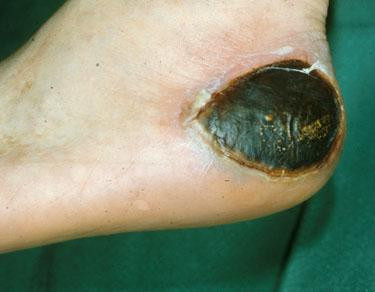
\includegraphics[width=0.7in]{gambar/dataset_citra/luka_hitam/2.jpg}&
		375x292\\
		\hline
		
		& &  &  \\
		2 & 
		luka\_hitam/4.jpg &
		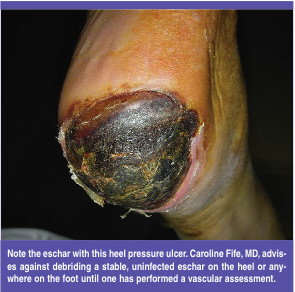
\includegraphics[width=0.7in]{gambar/dataset_citra/luka_hitam/4.jpg}&
		295x292\\
		\hline
		
		& &  &  \\
		3 & 
		luka\_hitam/5.jpg &
		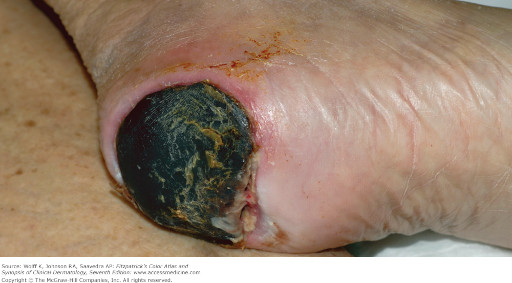
\includegraphics[width=0.7in]{gambar/dataset_citra/luka_hitam/5.jpg}&
		512x283\\
		\hline
		
		& &  &  \\
		4& 
		luka\_hitam/6.jpg &
		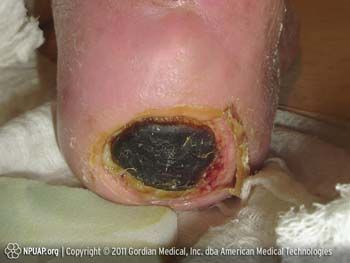
\includegraphics[width=0.7in]{gambar/dataset_citra/luka_hitam/6.jpg}&
		350x263\\
		\hline
		
		& &  &  \\
		5& 
		luka\_hitam/7.jpg &
		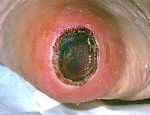
\includegraphics[width=0.7in]{gambar/dataset_citra/luka_hitam/7.jpg}&
		150x115\\
		\hline
		
		& &  &  \\
		6& 
		luka\_hitam/8.jpg &
		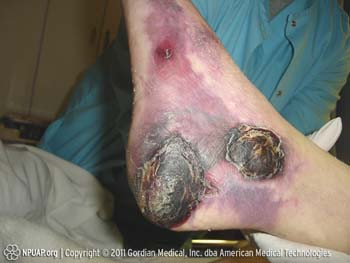
\includegraphics[width=0.7in]{gambar/dataset_citra/luka_hitam/8.jpg}&
		350x263\\
		\hline
		
		& &  &  \\
		7& 
		luka\_hitam/14.jpg &
		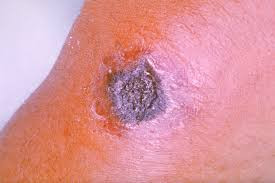
\includegraphics[width=0.7in]{gambar/dataset_citra/luka_hitam/14.jpg}&
		275x183\\
		\hline

		& &  &  \\
		8 & 
		luka\_hitam/15.jpg &
		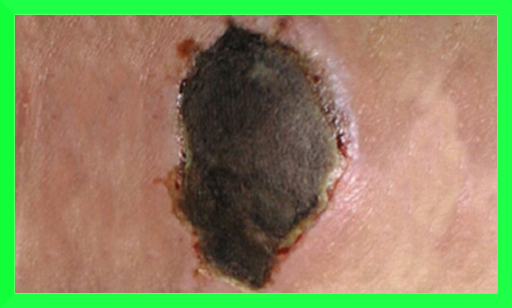
\includegraphics[width=0.7in]{gambar/dataset_citra/luka_hitam/15.jpg}&
		512x308\\
		\hline
		
		& &  &  \\
		9 & 
		luka\_hitam/17.jpg &
		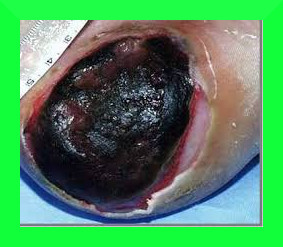
\includegraphics[width=0.7in]{gambar/dataset_citra/luka_hitam/17.jpg}&
		283x247\\
		\hline
	\end{tabular}
\end{table}

\begin{table}[H]
	\centering
	\caption{Visualisasi hasil pengolahan data citra input luka hitam - lanjutan}
	\label{tabel_input_2}
	\begin{tabular}{|m{0.2in}|m{1.2in}|m{0.7in}|m{0.7in}|}
		\hline
		\textbf{No} & \textbf{File} & \textbf{Citra} & \textbf{resolusi} \\
		\hline
		
		& &  &  \\
		10 & 
		luka\_hitam/18.jpg &
		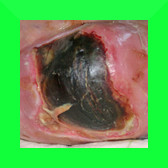
\includegraphics[width=0.7in]{gambar/dataset_citra/luka_hitam/18.jpg}&
		168x168\\
		\hline
		
		& &  &  \\
		11& 
		luka\_hitam/19.jpg &
		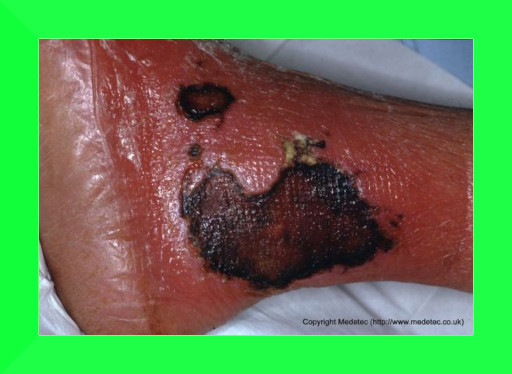
\includegraphics[width=0.7in]{gambar/dataset_citra/luka_hitam/19.jpg}&
		512x374\\
		\hline
		
		& &  &  \\
		12& 
		luka\_hitam/20.jpg &
		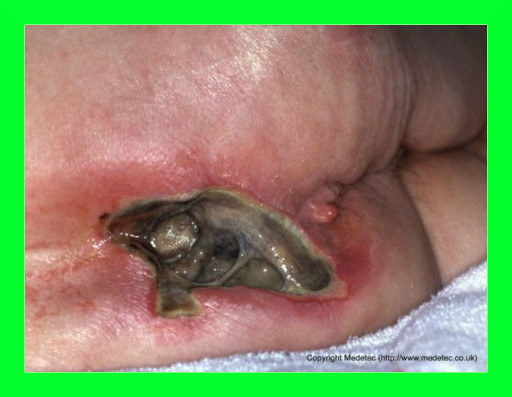
\includegraphics[width=0.7in]{gambar/dataset_citra/luka_hitam/20.jpg}&
		512x397\\
		\hline
		
		& &  &  \\
		13& 
		luka\_hitam/22.jpg &
		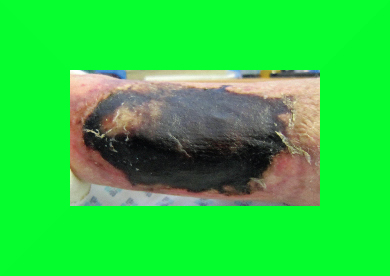
\includegraphics[width=0.7in]{gambar/dataset_citra/luka_hitam/22.jpg}&
		390x276\\
		\hline
		
		& &  &  \\
		14& 
		luka\_hitam/26.jpg &
		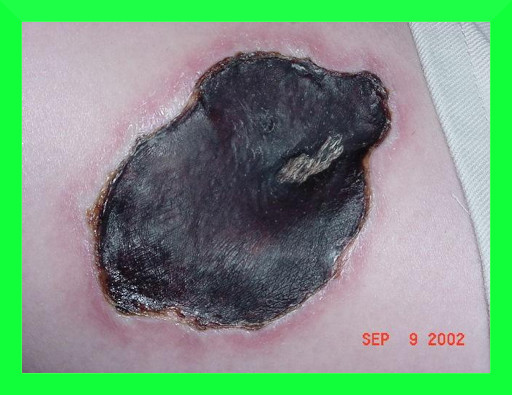
\includegraphics[width=0.7in]{gambar/dataset_citra/luka_hitam/26.jpg}&
		512x395\\
		\hline

		& &  &  \\
		15 & 
		luka\_hitam/27.jpg &
		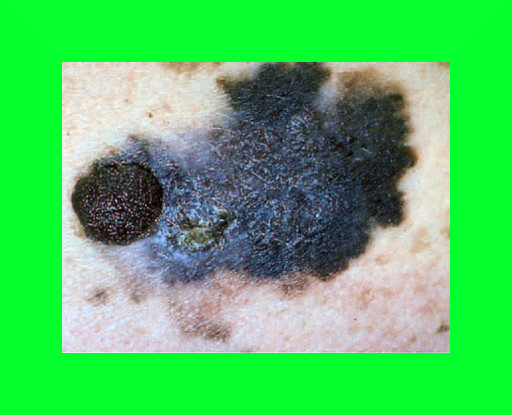
\includegraphics[width=0.7in]{gambar/dataset_citra/luka_hitam/27.jpg}&
		512x415\\
		\hline
		
		& &  &  \\
		16 & 
		luka\_hitam/28.jpg &
		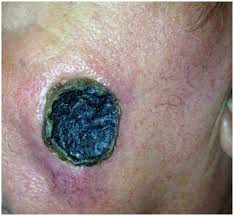
\includegraphics[width=0.7in]{gambar/dataset_citra/luka_hitam/28.jpg}&
		234x216\\
		\hline
		
		& &  &  \\
		17 & 
		luka\_hitam/29.jpg &
		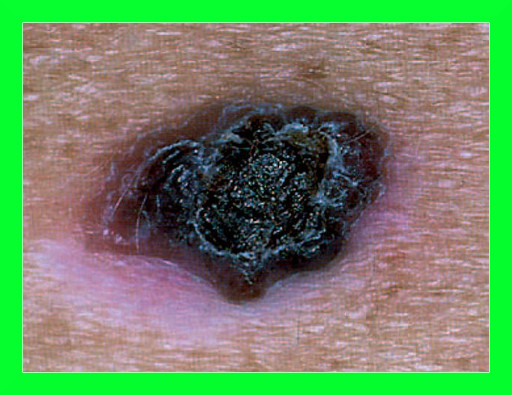
\includegraphics[width=0.7in]{gambar/dataset_citra/luka_hitam/29.jpg}&
		512x395\\
		\hline
	
		& &  &  \\
		18& 
		luka\_hitam/33.jpg &
		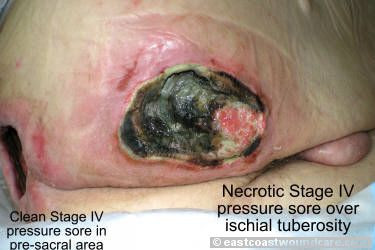
\includegraphics[width=0.7in]{gambar/dataset_citra/luka_hitam/33.jpg}&
		375x250\\
		\hline

	\end{tabular}
\end{table}

\begin{table}[H]
	\centering
	\caption{Visualisasi hasil pengolahan data citra input luka hitam - lanjutan}
	\label{tabel_input_3}
	\begin{tabular}{|m{0.2in}|m{1.2in}|m{0.7in}|m{0.7in}|}
		\hline
		\textbf{No} & \textbf{File} & \textbf{Citra} & \textbf{resolusi} \\
		\hline

		& &  &  \\
		19& 
		luka\_hitam/37.jpg &
		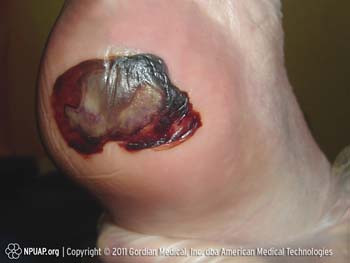
\includegraphics[width=0.7in]{gambar/dataset_citra/luka_hitam/37.jpg}&
		350x263\\
		\hline
		
		& &  &  \\
		20& 
		luka\_hitam/40.jpg &
		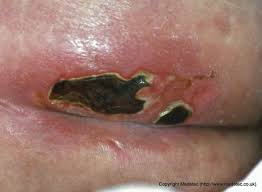
\includegraphics[width=0.7in]{gambar/dataset_citra/luka_hitam/40.jpg}&
		262x192\\
		\hline
		
		& &  &  \\
		21& 
		luka\_hitam/41.jpg &
		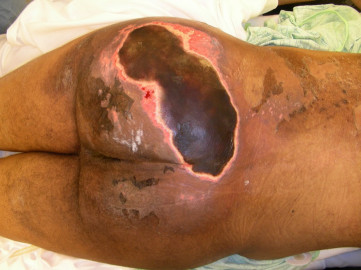
\includegraphics[width=0.7in]{gambar/dataset_citra/luka_hitam/41.jpg}&
		361x270\\
		\hline

		& &  &  \\
		22 & 
		luka\_hitam/16.jpg &
		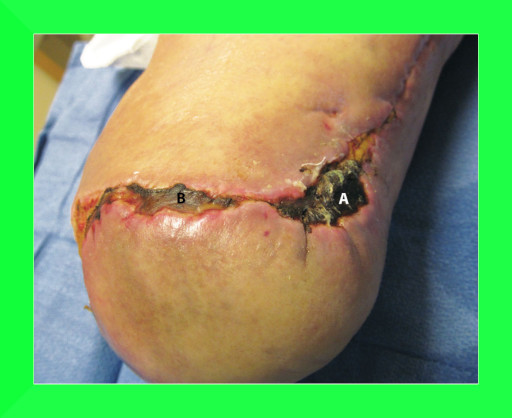
\includegraphics[width=0.7in]{gambar/dataset_citra/luka_hitam/16.jpg}&
		512x418\\
		\hline
		
		& &  &  \\
		23 & 
		luka\_hitam/31.jpg &
		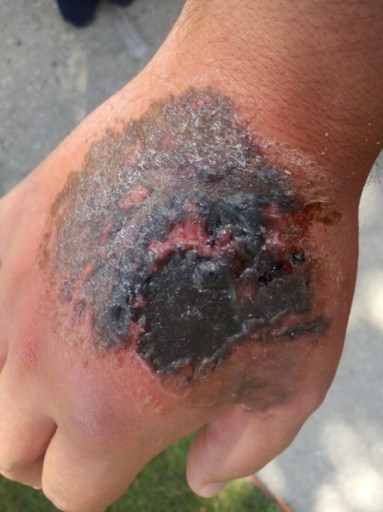
\includegraphics[width=0.7in]{gambar/dataset_citra/luka_hitam/31.jpg}&
		383x512\\
		\hline
		
		& &  &  \\
		24 & 
		luka\_hitam/39.jpg &
		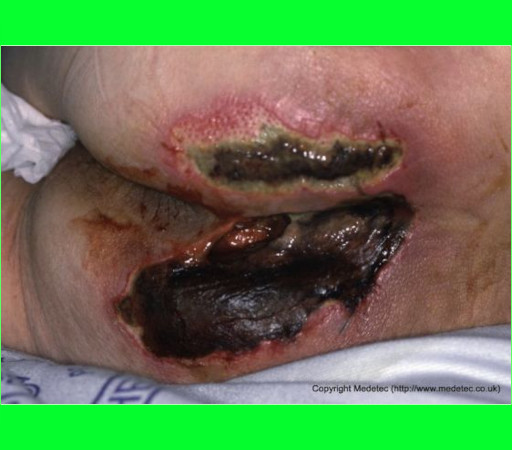
\includegraphics[width=0.7in]{gambar/dataset_citra/luka_hitam/39.jpg}&
		512x450\\
		\hline

	\end{tabular}
\end{table}

\begin{table}[H]
	\centering
	\caption{Visualisasi hasil pengolahan data citra input luka kuning}
	\label{tabel_input_5}
	\begin{tabular}{|m{0.2in}|m{1.2in}|m{0.7in}|m{0.7in}|}
		\hline
		\textbf{No} & \textbf{File} & \textbf{Citra} & \textbf{resolusi} \\
		\hline
		
		& &  &  \\
		1 & 
		luka\_kuning/13.jpg &
		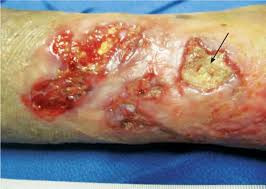
\includegraphics[width=0.7in]{gambar/dataset_citra/luka_kuning/13.jpg}&
		266x189\\
		\hline
		
		& &  &  \\
		2& 
		luka\_kuning/17.jpg &
		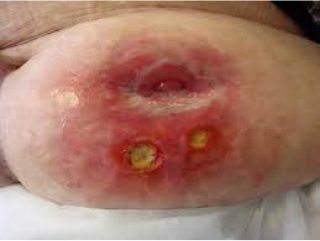
\includegraphics[width=0.7in]{gambar/dataset_citra/luka_kuning/17.jpg}&
		259x194\\
		\hline
		
		& &  &  \\
		3& 
		luka\_kuning/18.jpg &
		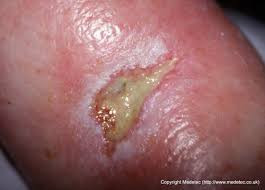
\includegraphics[width=0.7in]{gambar/dataset_citra/luka_kuning/18.jpg}&
		265x190\\
		\hline
		
		& &  &  \\
		4& 
		luka\_kuning/19.jpg &
		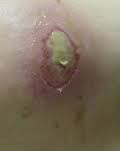
\includegraphics[width=0.7in]{gambar/dataset_citra/luka_kuning/19.jpg}&
		120x151\\
		\hline
		
		& &  &  \\
		5& 
		luka\_kuning/21.jpg &
		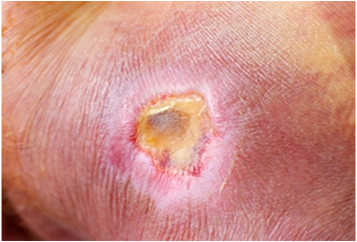
\includegraphics[width=0.7in]{gambar/dataset_citra/luka_kuning/21.jpg}&
		357x242\\
		\hline
		
		& &  &  \\
		6& 
		luka\_kuning/23.jpg &
		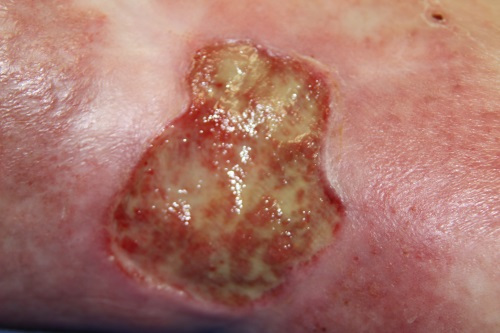
\includegraphics[width=0.7in]{gambar/dataset_citra/luka_kuning/23.jpg}&
		500x333\\
		\hline
		
		& &  &  \\
		7& 
		luka\_kuning/25.jpg &
		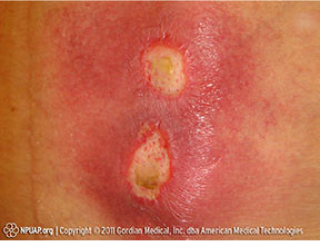
\includegraphics[width=0.7in]{gambar/dataset_citra/luka_kuning/25.jpg}&
		288x216\\
		\hline
				
		& &  &  \\
		8 & 
		luka\_kuning/34.jpg &
		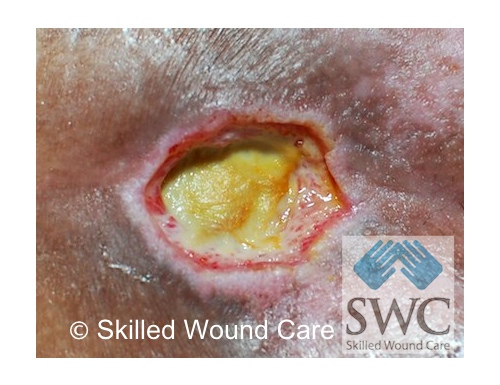
\includegraphics[width=0.7in]{gambar/dataset_citra/luka_kuning/34.jpg}&
		500x385\\
		\hline
		
		& &  &  \\
		9& 
		luka\_kuning/35.jpg &
		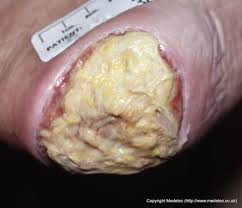
\includegraphics[width=0.7in]{gambar/dataset_citra/luka_kuning/35.jpg}&
		242x208\\
		\hline
		
		& &  &  \\
		10& 
		luka\_kuning/38.jpg &
		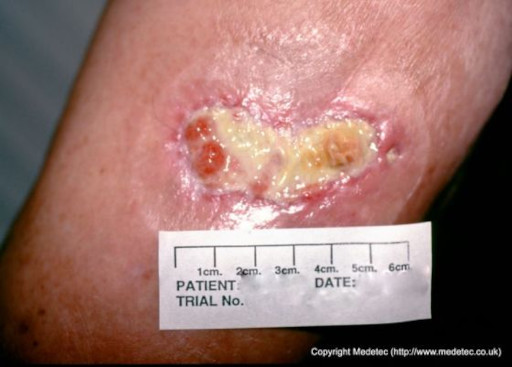
\includegraphics[width=0.7in]{gambar/dataset_citra/luka_kuning/38.jpg}&
		512x367\\
		\hline

	\end{tabular}
\end{table}

\begin{table}[H]
	\centering
	\caption{Visualisasi hasil pengolahan data citra input luka kuning - lanjutan}
	\label{tabel_input_6}
	\begin{tabular}{|m{0.2in}|m{1.2in}|m{0.7in}|m{0.7in}|}
		\hline
		\textbf{No} & \textbf{File} & \textbf{Citra} & \textbf{resolusi} \\
		\hline
		
		& &  &  \\
		11& 
		luka\_kuning/42.jpg &
		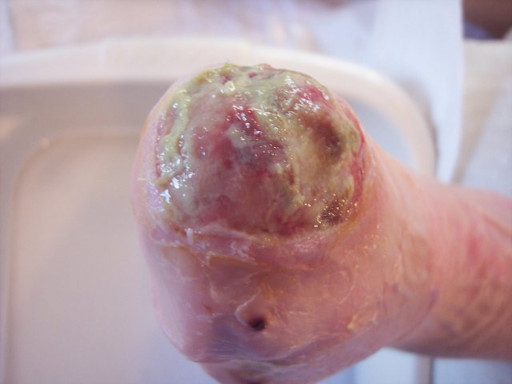
\includegraphics[width=0.7in]{gambar/dataset_citra/luka_kuning/42.jpg}&
		512x384\\
		\hline
		
		& &  &  \\
		12& 
		luka\_kuning/3.jpg &
		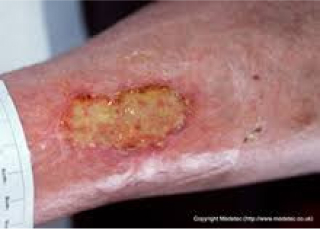
\includegraphics[width=0.7in]{gambar/dataset_citra/luka_kuning/3.jpg}&
		220x157\\
		\hline
		
		& &  &  \\
		13& 
		luka\_kuning/12.jpg &
		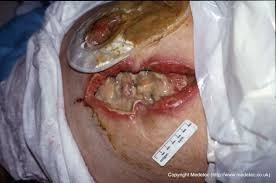
\includegraphics[width=0.7in]{gambar/dataset_citra/luka_kuning/12.jpg}&
		500x333\\
		\hline
		
		& &  &  \\
		14& 
		luka\_kuning/10.jpg &
		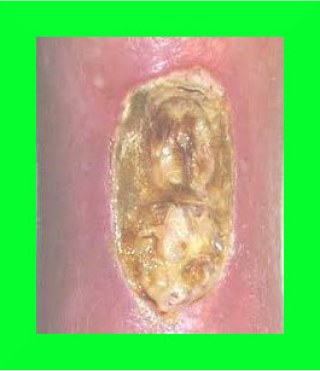
\includegraphics[width=0.7in]{gambar/dataset_citra/luka_kuning/10.jpg}&
		276x183\\
		\hline
				
		& &  &  \\
		15 & 
		luka\_kuning/16.jpg &
		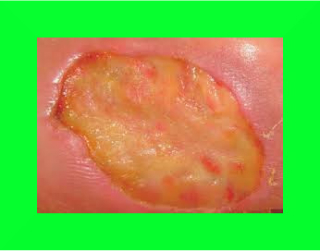
\includegraphics[width=0.7in]{gambar/dataset_citra/luka_kuning/16.jpg}&
		346x270\\
		\hline
	\end{tabular}
\end{table}

\begin{table}[H]
	\centering
	\caption{Visualisasi hasil pengolahan data citra input luka merah}
	\label{tabel_input_8}
	\begin{tabular}{|m{0.2in}|m{1.2in}|m{0.7in}|m{0.7in}|}
		\hline
		\textbf{No} & \textbf{File} & \textbf{Citra} & \textbf{resolusi} \\
		\hline
		
		& &  &  \\
		1 & 
		luka\_merah/16.jpg &
		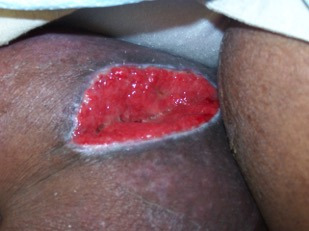
\includegraphics[width=0.7in]{gambar/dataset_citra/luka_merah/16.jpg}&
		309x231\\
		\hline
		
		& &  &  \\
		2& 
		luka\_merah/17.jpg &
		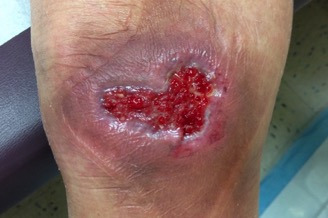
\includegraphics[width=0.7in]{gambar/dataset_citra/luka_merah/17.jpg}&
		328x218\\
		\hline
		
		& &  &  \\
		3& 
		luka\_merah/22.jpg &
		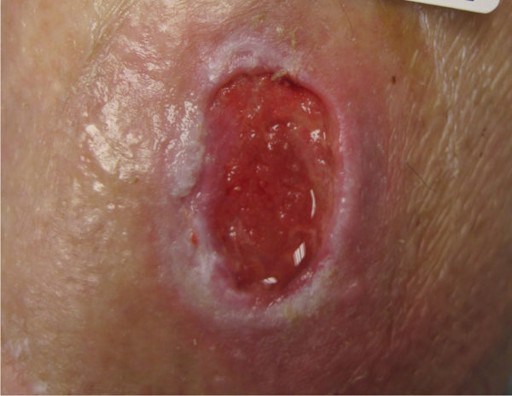
\includegraphics[width=0.7in]{gambar/dataset_citra/luka_merah/22.jpg}&
		512x396\\
		\hline
		
		& &  &  \\
		4& 
		luka\_merah/24.jpg &
		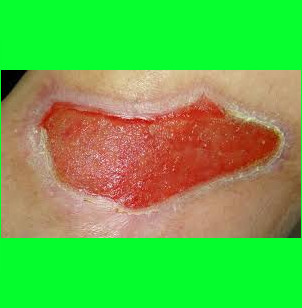
\includegraphics[width=0.7in]{gambar/dataset_citra/luka_merah/24.jpg}&
		302x308\\
		\hline
		
		& &  &  \\
		5& 
		luka\_merah/25.jpg &
		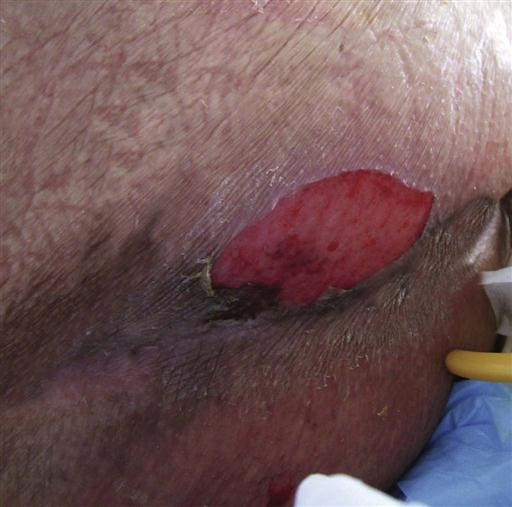
\includegraphics[width=0.7in]{gambar/dataset_citra/luka_merah/25.jpg}&
		512x507\\
		\hline
		
		& &  &  \\
		6& 
		luka\_merah/30.jpg &
		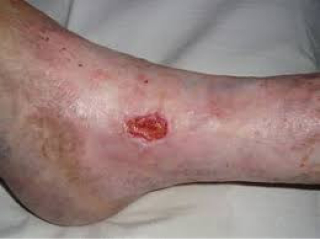
\includegraphics[width=0.7in]{gambar/dataset_citra/luka_merah/30.jpg}&
		260x194\\
		\hline
		
		& &  &  \\
		7& 
		luka\_merah/32.jpg &
		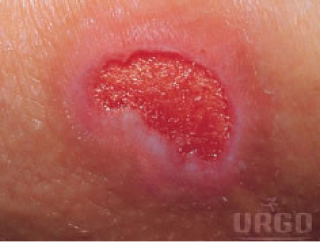
\includegraphics[width=0.7in]{gambar/dataset_citra/luka_merah/32.jpg}&
		236x178\\
		\hline

			
		& &  &  \\
		8 & 
		luka\_merah/33.jpg &
		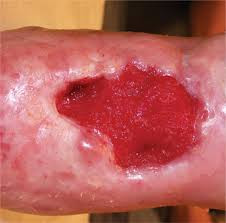
\includegraphics[width=0.7in]{gambar/dataset_citra/luka_merah/33.jpg}&
		226x223\\
		\hline
		
		& &  &  \\
		9& 
		luka\_merah/37.jpg &
		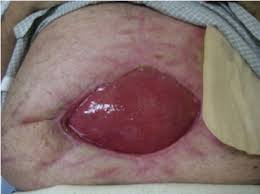
\includegraphics[width=0.7in]{gambar/dataset_citra/luka_merah/37.jpg}&
		260x194\\
		\hline
		
		& &  &  \\
		10& 
		luka\_merah/39.jpg &
		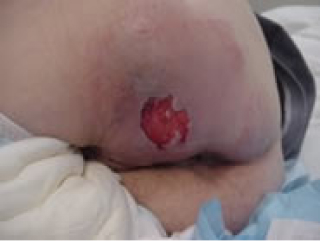
\includegraphics[width=0.7in]{gambar/dataset_citra/luka_merah/39.jpg}&
		185x139\\
		\hline

	\end{tabular}
\end{table}

\begin{table}[H]
	\centering
	\caption{Visualisasi hasil pengolahan data citra input luka merah - lanjutan}
	\label{tabel_input_9}
	\begin{tabular}{|m{0.2in}|m{1.2in}|m{0.7in}|m{0.7in}|}
		\hline
		\textbf{No} & \textbf{File} & \textbf{Citra} & \textbf{resolusi} \\
		\hline
		
		& &  &  \\
		11& 
		luka\_merah/42.jpg &
		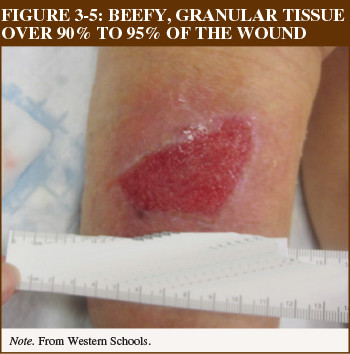
\includegraphics[width=0.7in]{gambar/dataset_citra/luka_merah/42.jpg}&
		350x354\\
		\hline
		
		& &  &  \\
		12& 
		luka\_merah/44.jpg &
		\includegraphics[width=0.7in]{gambar/dataset_citra/luka_merah/44.jpg}&
		512x363\\
		\hline
		
		& &  &  \\
		13& 
		luka\_merah/2.jpg &
		\includegraphics[width=0.7in]{gambar/dataset_citra/luka_merah/2.jpg}&
		288x512\\
		\hline
		
		& &  &  \\
		14& 
		luka\_merah/3.jpg &
		\includegraphics[width=0.7in]{gambar/dataset_citra/luka_merah/3.jpg}&
		384x512\\
		\hline

		& &  &  \\
		15 & 
		luka\_merah/4.jpg &
		\includegraphics[width=0.7in]{gambar/dataset_citra/luka_merah/4.jpg}&
		384x512\\
		\hline
		
		& &  &  \\
		16& 
		luka\_merah/6.jpg &
		\includegraphics[width=0.7in]{gambar/dataset_citra/luka_merah/6.jpg}&
		512x384\\
		\hline
		
		& &  &  \\
		17& 
		luka\_merah/7.jpg &
		\includegraphics[width=0.7in]{gambar/dataset_citra/luka_merah/7.jpg}&
		512x341\\
		\hline
		
		& &  &  \\
		18& 
		luka\_merah/8.jpg &
		\includegraphics[width=0.7in]{gambar/dataset_citra/luka_merah/8.jpg}&
		512x384\\
		\hline
		
	\end{tabular}
\end{table}

\begin{table}[H]
	\centering
	\caption{Visualisasi hasil pengolahan data citra input luka merah - lanjutan}
	\label{tabel_input_10}
	\begin{tabular}{|m{0.2in}|m{1.2in}|m{0.7in}|m{0.7in}|}
		\hline
		\textbf{No} & \textbf{File} & \textbf{Citra} & \textbf{resolusi} \\
		\hline
			
		& &  &  \\
		19& 
		luka\_merah/9.jpg &
		\includegraphics[width=0.7in]{gambar/dataset_citra/luka_merah/9.jpg}&
		288x512\\
		\hline
		
		& &  &  \\
		20& 
		luka\_merah/10.jpg &
		\includegraphics[width=0.7in]{gambar/dataset_citra/luka_merah/10.jpg}&
		512x384\\
		\hline
		
		& &  &  \\
		21& 
		luka\_merah/11.jpg &
		\includegraphics[width=0.7in]{gambar/dataset_citra/luka_merah/11.jpg}&
		512x384\\
		\hline

		& &  &  \\
		22 & 
		luka\_merah/12.jpg &
		\includegraphics[width=0.7in]{gambar/dataset_citra/luka_merah/12.jpg}&
		512x384\\
		\hline
		
		& &  &  \\
		23& 
		luka\_merah/14.jpg &
		\includegraphics[width=0.7in]{gambar/dataset_citra/luka_merah/14.jpg}&
		512x384\\
		\hline
		
		& &  &  \\
		24& 
		luka\_merah/18.jpg &
		\includegraphics[width=0.7in]{gambar/dataset_citra/luka_merah/18.jpg}&
		512x382\\
		\hline
		
		& &  &  \\
		25& 
		luka\_merah/19.jpg &
		\includegraphics[width=0.7in]{gambar/dataset_citra/luka_merah/19.jpg}&
		512x458\\
		\hline
		
		& &  &  \\
		26& 
		luka\_merah/20.jpg &
		\includegraphics[width=0.7in]{gambar/dataset_citra/luka_merah/20.jpg}&
		408x360\\
		\hline

	\end{tabular}
\end{table}

\begin{table}[H]
	\centering
	\caption{Visualisasi hasil pengolahan data citra input luka merah - lanjutan}
	\label{tabel_input_12}
	\begin{tabular}{|m{0.2in}|m{1.2in}|m{0.7in}|m{0.7in}|}
		\hline
		\textbf{No} & \textbf{File} & \textbf{Citra} & \textbf{resolusi} \\
		\hline

		& &  &  \\
		27& 
		luka\_merah/23.jpg &
		\includegraphics[width=0.7in]{gambar/dataset_citra/luka_merah/23.jpg}&
		512x384\\
		\hline
		
		& &  &  \\
		28& 
		luka\_merah/26.jpg &
		\includegraphics[width=0.7in]{gambar/dataset_citra/luka_merah/26.jpg}&
		512x464\\
		\hline
		
		& &  &  \\
		29 & 
		luka\_merah/29.jpg &
		\includegraphics[width=0.7in]{gambar/dataset_citra/luka_merah/29.jpg}&
		328x218\\
		\hline
		
		& &  &  \\
		29& 
		luka\_merah/35.jpg &
		\includegraphics[width=0.7in]{gambar/dataset_citra/luka_merah/35.jpg}&
		261x295\\
		\hline
		
		& &  &  \\
		30& 
		luka\_merah/36.jpg &
		\includegraphics[width=0.7in]{gambar/dataset_citra/luka_merah/36.jpg}&
		295x194\\
		\hline
		
		& &  &  \\
		31& 
		luka\_merah/38.jpg &
		\includegraphics[width=0.7in]{gambar/dataset_citra/luka_merah/38.jpg}&
		512x384\\
		\hline
		
		& &  &  \\
		32& 
		luka\_merah/20.jpg &
		\includegraphics[width=0.7in]{gambar/dataset_citra/luka_merah/20.jpg}&
		408x360\\
		\hline
	\end{tabular}
\end{table}

\chapter{Tabel hasil deteksi keliling luka menggunakan \emph{Grabcut}}

\begin{table}[H]
	\centering
	\caption{Visualisasi hasil deteksi keliling luka hitam menggunakan \emph{Grabcut}}
	\label{tabel_hasil_1}
	\begin{tabular}{|m{1.0in}|m{1.0in}|m{1.0in}|m{1.0in}|m{0.6in}|}
		\hline
		\textbf{Inisialisasi Bounding Box} & \textbf{Hasil Segmentasi} & \textbf{Hasil Area Akhir} & \textbf{Area \emph{Ground Truth}} & \textbf{Akurasi} \\
		\hline
		
		&  &  & \\
		\includegraphics[width=1.0in]{gambar/hasil_segmentasi/luka_hitam/image_2_rect.jpg} {\centering\fontsize{10}{10}\selectfont(153,48,299,158)}&
		\includegraphics[width=1.0in]{gambar/hasil_segmentasi/luka_hitam/result_2.jpg}&
		\includegraphics[width=1.0in]{gambar/hasil_segmentasi/luka_hitam/mask_r_2.jpg}&
		\includegraphics[width=1.0in]{gambar/hasil_segmentasi/luka_hitam/2_r.jpg}&
		95.36\% \\
		\hline

		&  &  & \\
		\includegraphics[width=1.0in]{gambar/hasil_segmentasi/luka_hitam/image_4_rect.jpg} {\centering\fontsize{10}{10}\selectfont(60,89,162,153)}&
		\includegraphics[width=1.0in]{gambar/hasil_segmentasi/luka_hitam/result_4.jpg}&
		\includegraphics[width=1.0in]{gambar/hasil_segmentasi/luka_hitam/mask_r_4.jpg}&
		\includegraphics[width=1.0in]{gambar/hasil_segmentasi/luka_hitam/4_r.jpg}&
		95.15\% \\
		\hline
		
		&  &  & \\
		\includegraphics[width=1.0in]{gambar/hasil_segmentasi/luka_hitam/image_5_rect.jpg} {\centering\fontsize{10}{10}\selectfont(68,48,115,106)}&
		\includegraphics[width=1.0in]{gambar/hasil_segmentasi/luka_hitam/result_5.jpg}&
		\includegraphics[width=1.0in]{gambar/hasil_segmentasi/luka_hitam/mask_r_5.jpg}&
		\includegraphics[width=1.0in]{gambar/hasil_segmentasi/luka_hitam/5_r.jpg}&
		95.34\% \\
		\hline
		
		&  &  & \\
		\includegraphics[width=1.0in]{gambar/hasil_segmentasi/luka_hitam/image_6_rect.jpg} {\centering\fontsize{10}{10}\selectfont(83,97,130,97)}&
		\includegraphics[width=1.0in]{gambar/hasil_segmentasi/luka_hitam/result_6.jpg}&
		\includegraphics[width=1.0in]{gambar/hasil_segmentasi/luka_hitam/mask_r_6.jpg}&
		\includegraphics[width=1.0in]{gambar/hasil_segmentasi/luka_hitam/6_r.jpg}&
		93.74\% \\
		\hline
		
	\end{tabular}
\end{table}

\begin{table}[H]
	\centering
	\caption{Visualisasi hasil deteksi keliling luka hitam menggunakan \emph{Grabcut}}
	\label{tabel_hasil_2}
	\begin{tabular}{|m{1.0in}|m{1.0in}|m{1.0in}|m{1.0in}|m{0.6in}|}
		\hline
		\textbf{Inisialisasi Bounding Box} & \textbf{Hasil Segmentasi} & \textbf{Hasil Citra Referensi} & \textbf{Area Segmentasi} & \textbf{Akurasi} \\
		\hline

		&  &  & \\
		\includegraphics[width=1.0in]{gambar/hasil_segmentasi/luka_hitam/image_7_rect.jpg} {\centering\fontsize{10}{10}\selectfont(100,50,117,142)}&
		\includegraphics[width=1.0in]{gambar/hasil_segmentasi/luka_hitam/result_7.jpg}&
		\includegraphics[width=1.0in]{gambar/hasil_segmentasi/luka_hitam/mask_r_7.jpg}&
		\includegraphics[width=1.0in]{gambar/hasil_segmentasi/luka_hitam/7_r.jpg}&
		92.97\% \\
		\hline
		
		&  &  & \\
		\includegraphics[width=1.0in]{gambar/hasil_segmentasi/luka_hitam/image_8_rect.jpg} {\centering\fontsize{10}{10}\selectfont(114,104,157,108)}&
		\includegraphics[width=1.0in]{gambar/hasil_segmentasi/luka_hitam/result_8.jpg}&
		\includegraphics[width=1.0in]{gambar/hasil_segmentasi/luka_hitam/mask_r_8.jpg}&
		\includegraphics[width=1.0in]{gambar/hasil_segmentasi/luka_hitam/8_r.jpg}&
		83.35\% \\
		\hline
		
		&  &  & \\
		\includegraphics[width=1.0in]{gambar/hasil_segmentasi/luka_hitam/image_14_rect.jpg} {\centering\fontsize{10}{10}\selectfont(98,43,116,121)}&
		\includegraphics[width=1.0in]{gambar/hasil_segmentasi/luka_hitam/result_14.jpg}&
		\includegraphics[width=1.0in]{gambar/hasil_segmentasi/luka_hitam/mask_r_14.jpg}&
		\includegraphics[width=1.0in]{gambar/hasil_segmentasi/luka_hitam/14_r.jpg}&
		88.89\% \\
		\hline
		
		&  &  & \\
		\includegraphics[width=1.0in]{gambar/hasil_segmentasi/luka_hitam/image_15_rect.jpg} {\centering\fontsize{10}{10}\selectfont(89,10,140,171)}&
		\includegraphics[width=1.0in]{gambar/hasil_segmentasi/luka_hitam/result_15.jpg}&
		\includegraphics[width=1.0in]{gambar/hasil_segmentasi/luka_hitam/mask_r_15.jpg}&
		\includegraphics[width=1.0in]{gambar/hasil_segmentasi/luka_hitam/15_r.jpg}&
		91.78\% \\
		\hline
		
		&  &  & \\
		\includegraphics[width=1.0in]{gambar/hasil_segmentasi/luka_hitam/image_17_rect.jpg} {\centering\fontsize{10}{10}\selectfont(28,34,208,213)}&
		\includegraphics[width=1.0in]{gambar/hasil_segmentasi/luka_hitam/result_17.jpg}&
		\includegraphics[width=1.0in]{gambar/hasil_segmentasi/luka_hitam/mask_r_17.jpg}&
		\includegraphics[width=1.0in]{gambar/hasil_segmentasi/luka_hitam/17_r.jpg}&
		87.58\% \\
		\hline

	\end{tabular}
\end{table}

\begin{table}[H]
	\centering
	\caption{Visualisasi hasil deteksi keliling luka hitam menggunakan \emph{Grabcut}}
	\label{tabel_hasil_3}
	\begin{tabular}{|m{1.0in}|m{1.0in}|m{1.0in}|m{1.0in}|m{0.6in}|}
		\hline
		\textbf{Inisialisasi Bounding Box} & \textbf{Hasil Segmentasi} & \textbf{Hasil Citra Referensi} & \textbf{Area Segmentasi} & \textbf{Akurasi} \\
		\hline
		
		&  &  & \\
		\includegraphics[width=1.0in]{gambar/hasil_segmentasi/luka_hitam/image_18_rect.jpg} {\centering\fontsize{10}{10}\selectfont(50,59,219,201)}&
		\includegraphics[width=1.0in]{gambar/hasil_segmentasi/luka_hitam/result_18.jpg}&
		\includegraphics[width=1.0in]{gambar/hasil_segmentasi/luka_hitam/mask_r_18.jpg}&
		\includegraphics[width=1.0in]{gambar/hasil_segmentasi/luka_hitam/18_r.jpg}&
		91.42\% \\
		\hline

		&  &  & \\
		\includegraphics[width=1.0in]{gambar/hasil_segmentasi/luka_hitam/image_19_rect.jpg} {\centering\fontsize{10}{10}\selectfont(107,82,147,104)}&
		\includegraphics[width=1.0in]{gambar/hasil_segmentasi/luka_hitam/result_19.jpg}&
		\includegraphics[width=1.0in]{gambar/hasil_segmentasi/luka_hitam/mask_r_19.jpg}&
		\includegraphics[width=1.0in]{gambar/hasil_segmentasi/luka_hitam/19_r.jpg}&
		94.34\% \\
		\hline
		
		&  &  & \\
		\includegraphics[width=1.0in]{gambar/hasil_segmentasi/luka_hitam/image_20_rect.jpg} {\centering\fontsize{10}{10}\selectfont(51,107,168,101)}&
		\includegraphics[width=1.0in]{gambar/hasil_segmentasi/luka_hitam/result_20.jpg}&
		\includegraphics[width=1.0in]{gambar/hasil_segmentasi/luka_hitam/mask_r_20.jpg}&
		\includegraphics[width=1.0in]{gambar/hasil_segmentasi/luka_hitam/20_r.jpg}&
		93.78\% \\
		\hline
		
		&  &  & \\
		\includegraphics[width=1.0in]{gambar/hasil_segmentasi/luka_hitam/image_22_rect.jpg} {\centering\fontsize{10}{10}\selectfont(63,67,186,98)}&
		\includegraphics[width=1.0in]{gambar/hasil_segmentasi/luka_hitam/result_22.jpg}&
		\includegraphics[width=1.0in]{gambar/hasil_segmentasi/luka_hitam/mask_r_22.jpg}&
		\includegraphics[width=1.0in]{gambar/hasil_segmentasi/luka_hitam/22_r.jpg}&
		92.52\% \\
		\hline 
				
		&  &  & \\
		\includegraphics[width=1.0in]{gambar/hasil_segmentasi/luka_hitam/image_26_rect.jpg} {\centering\fontsize{10}{10}\selectfont(63,67,186,98)}&
		\includegraphics[width=1.0in]{gambar/hasil_segmentasi/luka_hitam/result_26.jpg}&
		\includegraphics[width=1.0in]{gambar/hasil_segmentasi/luka_hitam/mask_r_26.jpg}&
		\includegraphics[width=1.0in]{gambar/hasil_segmentasi/luka_hitam/26_r.jpg}&
		94.01\% \\
		\hline 

		&  &  & \\
		\includegraphics[width=1.0in]{gambar/hasil_segmentasi/luka_hitam/image_27_rect.jpg} {\centering\fontsize{10}{10}\selectfont(63,67,186,98)}&
		\includegraphics[width=1.0in]{gambar/hasil_segmentasi/luka_hitam/result_27.jpg}&
		\includegraphics[width=1.0in]{gambar/hasil_segmentasi/luka_hitam/mask_r_27.jpg}&
		\includegraphics[width=1.0in]{gambar/hasil_segmentasi/luka_hitam/27_r.jpg}&
		88.84\% \\
		\hline 

	\end{tabular}
\end{table}


\begin{table}[H]
	\centering
	\caption{Visualisasi hasil deteksi keliling luka hitam menggunakan \emph{Grabcut}}
	\label{tabel_hasil_4}
	\begin{tabular}{|m{1.0in}|m{1.0in}|m{1.0in}|m{1.0in}|m{0.6in}|}
		\hline
		\textbf{Inisialisasi Bounding Box} & \textbf{Hasil Segmentasi} & \textbf{Hasil Citra Referensi} & \textbf{Area Segmentasi} & \textbf{Akurasi} \\
		\hline
		
		&  &  & \\
		\includegraphics[width=1.0in]{gambar/hasil_segmentasi/luka_hitam/image_28_rect.jpg} {\centering\fontsize{10}{10}\selectfont(63,67,186,98)}&
		\includegraphics[width=1.0in]{gambar/hasil_segmentasi/luka_hitam/result_28.jpg}&
		\includegraphics[width=1.0in]{gambar/hasil_segmentasi/luka_hitam/mask_r_28.jpg}&
		\includegraphics[width=1.0in]{gambar/hasil_segmentasi/luka_hitam/28_r.jpg}&
		95.2\% \\
		\hline 

		&  &  & \\
		\includegraphics[width=1.0in]{gambar/hasil_segmentasi/luka_hitam/image_29_rect.jpg} {\centering\fontsize{10}{10}\selectfont(63,67,186,98)}&
		\includegraphics[width=1.0in]{gambar/hasil_segmentasi/luka_hitam/result_29.jpg}&
		\includegraphics[width=1.0in]{gambar/hasil_segmentasi/luka_hitam/mask_r_29.jpg}&
		\includegraphics[width=1.0in]{gambar/hasil_segmentasi/luka_hitam/29_r.jpg}&
		87.77\% \\
		\hline 

		&  &  & \\
		\includegraphics[width=1.0in]{gambar/hasil_segmentasi/luka_hitam/image_33_rect.jpg} {\centering\fontsize{10}{10}\selectfont(63,67,186,98)}&
		\includegraphics[width=1.0in]{gambar/hasil_segmentasi/luka_hitam/result_33.jpg}&
		\includegraphics[width=1.0in]{gambar/hasil_segmentasi/luka_hitam/mask_r_33.jpg}&
		\includegraphics[width=1.0in]{gambar/hasil_segmentasi/luka_hitam/33_r.jpg}&
		94.68\% \\
		\hline 

		&  &  & \\
		\includegraphics[width=1.0in]{gambar/hasil_segmentasi/luka_hitam/image_37_rect.jpg} {\centering\fontsize{10}{10}\selectfont(63,67,186,98)}&
		\includegraphics[width=1.0in]{gambar/hasil_segmentasi/luka_hitam/result_37.jpg}&
		\includegraphics[width=1.0in]{gambar/hasil_segmentasi/luka_hitam/mask_r_37.jpg}&
		\includegraphics[width=1.0in]{gambar/hasil_segmentasi/luka_hitam/37_r.jpg}&
		95.45\% \\
		\hline 

		&  &  & \\
		\includegraphics[width=1.0in]{gambar/hasil_segmentasi/luka_hitam/image_40_rect.jpg} {\centering\fontsize{10}{10}\selectfont(63,67,186,98)}&
		\includegraphics[width=1.0in]{gambar/hasil_segmentasi/luka_hitam/result_40.jpg}&
		\includegraphics[width=1.0in]{gambar/hasil_segmentasi/luka_hitam/mask_r_40.jpg}&
		\includegraphics[width=1.0in]{gambar/hasil_segmentasi/luka_hitam/40_r.jpg}&
		92.84\% \\
		\hline 

		&  &  & \\
		\includegraphics[width=1.0in]{gambar/hasil_segmentasi/luka_hitam/image_41_rect.jpg} {\centering\fontsize{10}{10}\selectfont(63,67,186,98)}&
		\includegraphics[width=1.0in]{gambar/hasil_segmentasi/luka_hitam/result_41.jpg}&
		\includegraphics[width=1.0in]{gambar/hasil_segmentasi/luka_hitam/mask_r_41.jpg}&
		\includegraphics[width=1.0in]{gambar/hasil_segmentasi/luka_hitam/41_r.jpg}&
		85.88\% \\
		\hline 

	\end{tabular}
\end{table}

\begin{table}[H]
	\centering
	\caption{Visualisasi hasil deteksi keliling luka hitam menggunakan \emph{Grabcut}}
	\label{tabel_hasil_5}
	\begin{tabular}{|m{1.0in}|m{1.0in}|m{1.0in}|m{1.0in}|m{0.6in}|}
		\hline
		\textbf{Inisialisasi Bounding Box} & \textbf{Hasil Segmentasi} & \textbf{Hasil Citra Referensi} & \textbf{Area Segmentasi} & \textbf{Akurasi} \\
		\hline

		&  &  & \\
		\includegraphics[width=1.0in]{gambar/hasil_segmentasi/luka_hitam/image_16_rect.jpg} {\centering\fontsize{10}{10}\selectfont(63,67,186,98)}&
		\includegraphics[width=1.0in]{gambar/hasil_segmentasi/luka_hitam/result_16.jpg}&
		\includegraphics[width=1.0in]{gambar/hasil_segmentasi/luka_hitam/mask_r_16.jpg}&
		\includegraphics[width=1.0in]{gambar/hasil_segmentasi/luka_hitam/16_r.jpg}&
		92.63\% \\
		\hline 

		&  &  & \\
		\includegraphics[width=1.0in]{gambar/hasil_segmentasi/luka_hitam/image_31_rect.jpg} {\centering\fontsize{10}{10}\selectfont(63,67,186,98)}&
		\includegraphics[width=1.0in]{gambar/hasil_segmentasi/luka_hitam/result_31.jpg}&
		\includegraphics[width=1.0in]{gambar/hasil_segmentasi/luka_hitam/mask_r_31.jpg}&
		\includegraphics[width=1.0in]{gambar/hasil_segmentasi/luka_hitam/31_r.jpg}&
		87.35\% \\
		\hline 

		&  &  & \\
		\includegraphics[width=1.0in]{gambar/hasil_segmentasi/luka_hitam/image_39_rect.jpg} {\centering\fontsize{10}{10}\selectfont(63,67,186,98)}&
		\includegraphics[width=1.0in]{gambar/hasil_segmentasi/luka_hitam/result_39.jpg}&
		\includegraphics[width=1.0in]{gambar/hasil_segmentasi/luka_hitam/mask_r_39.jpg}&
		\includegraphics[width=1.0in]{gambar/hasil_segmentasi/luka_hitam/39_r.jpg}&
		86.43\% \\
		\hline 


	\end{tabular}
\end{table}